\chapter{Event Generation, Simulation and Reconstruction}
\label{chap:Reconstruction}
Event simulation plays a significant role in the operation of any experiment. Before the real data taking, reconstruction algorithms, efficiency of trigger paths, analysis strategies and other operational details of the experiment need to be studied and optimized well. This is achieved by simulation of the apparatus and the expected processes using the Monte Carlo (MC) method \cite{Monte}. In high energy physics, the simulation of experimental data is done in two steps : event generation and detector simulation. Event generators simulate a collision starting from the proton-proton interaction up to the production of the final decay products, to be observed with the CMS detector. The output of an event generator is used as input for a detector simulation program which models the interactions of the generated final-state particles with the detector. This procedure requires a sophisticated and complex simulation of the detector material and of the behaviour of the particles in it.

\section{Event Generation and Simulation Software}
In real world, the machine or collider produces interactions which are observed by detectors. The interesting events are stored and reconstructed afterwards for a physics analysis. In the Monte Carlo world, the role of machines is played by the event generators. The event generators generate simulated events as detailed as observed by a detector. The output of an event generator is in the form of ``events'' with the same behaviour and fluctuations as real data which serves as an input to the detector simulation, allowing a precise prediction and verification for the entire system of experimental setup. The comparison of real and Monte Carlo world is presented in Fig.~\ref{fig:sim}. %There are a variety of Monte Carlo event generators which are commonly used in high energy physics. The MC event generators used in this thesis include leading order (LO) generators : \MadGraph, \PYTHIA~and \HERWIG~as well as the next-to-leading order generator \POWHEG. These generators are described one by one in the following sections.

\begin{figure}[h!]
\begin{center}
\vspace*{2mm} 
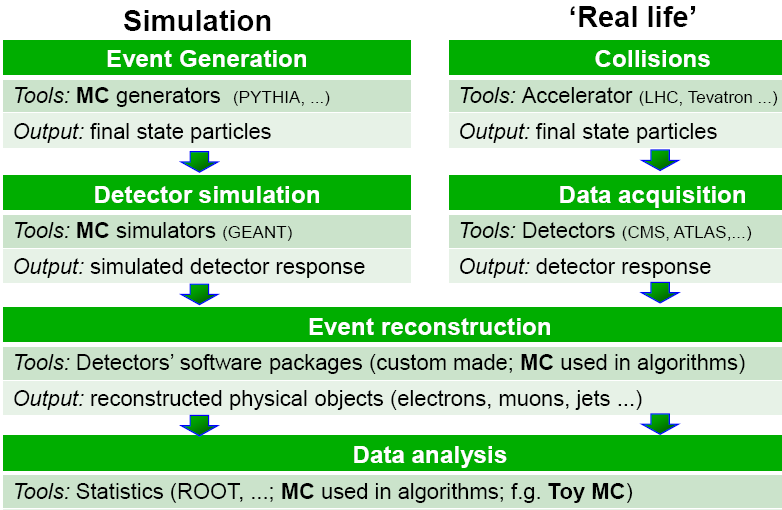
\includegraphics[scale = 0.7]{/home/anter/Desktop/Thesis/Figures/Simulation.png}\\
\vspace*{4mm} 
\caption{Comparison of Monte Carlo simulations with the real world data.}
\label{fig:sim}
\end{center}
\end{figure}

There are a variety of Monte Carlo event generators which are commonly used in high energy physics. The MC event generators used in this thesis include leading order (LO) generators : \PYTHIA, \MadGraphF and \HERWIG~as well as the next-to-leading order generator \POWHEG. These generators are described one by one in the following sections.

\subsection{\PYTHIA}
\PYTHIA~is the most widely used program to generate the collisions at high energies for p-p, e-e and e-p colliders. It contains theory and models for a number of physics aspects, including hard and soft processes, parton distributions, initial-state and final-state parton showers, multiple interactions, fragmentation and decay. It also has a set of utilities and interfaces to external programs. It uses the Lund string hadronization model \cite{Lund} to describe the hadronization process. \PYTHIA~was originally coded in FORTRAN language under the version 6 i.e. \PYTHIAS \cite{Sjostrand:2006za}. In 2004, it was rewritten in C\plusn\plus and was released as \PYTHIAE \cite{Sjostrand:2007gs} in 2007. The two versions differ in the description of multi-parton interactions. Both the versions use leading order (LO) calculations to derive the colored partons from the hard interaction. From these partons, colorless objects like hadrons, leptons and photons are produced. For the studies in this thesis, \PYTHIAS with tune \Ztwostar \cite{Field:2011iq} and \PYTHIAE with tunes CUETS1 and CUETM1 \cite{Khachatryan:2015pea} have been used. 

\subsection{\MadGraphF}
\MadGraphF~\cite{Alwall:2011uj} generates matrix elements for high energy physics processes, such as decays and $2 \rightarrow n$ scatterings. The event information of the hard process such as particle ID, momenta, spin etc. is stored in the Les Houches format \cite{Alwall:2006yp} and can be interfaced to other generators. In this thesis, \MadGraphF has been interfaced to \PYTHIAS with tune \Ztwostar to handle the rest of the generation steps which involves parton showering and hadronization. Matching algorithms make sure that thers is no double-counting between the tree-level and the PS-model-generated partons. \MadGraphFn\plusn \PYTHIAS (\MGP) samples are used mainly for general comparisons to data and calculating the detector resolution. 

\subsection{\HERWIG}
\HERWIG~(Hadron Emission Reactions With Interfering Gluons) \cite{Corcella:2000bw} is a multi-purpose event generator. It includes the simulation of hard lepton-lepton, lepton-hadron and hadron-hadron scattering and soft hadron-hadron collisions. It uses angular ordering for parton showers and cluster model for hadronization. The \HERWIG~generator includes a number of hard scattering processes and has the possibility to interface external matrix element generators. It uses angular ordering for parton showers and cluster model for hadronization. \HERWIG~was FORTRAN based and has a version in C\plusn\plusn, named \HERWIGPP \cite{Bahr:2008pv}. The samples generated using \HERWIGPP generator with the default tune of version 2.3 \cite{Bahr:2008tf} have been used to study non-perturbative effects. 

\subsection{\POWHEG}
\POWHEG generator performs the fixed next-to-leading order (NLO) calculations merged with parton showers \cite{Frixione:2007vw, Nason:2004rx, Alioli:2010xa}. A computer framework known as \POWHEG BOX \cite{Oleari:2010nx}, implements NLO calculations in shower Monte Carlo programs according to the \POWHEG method. It can be interfaced with all modern shower Monte Carlo programs that support the Les Houches Interface for User Generated Processes. It contains the hard matrix elements for NLO dijet production. For the parton shower and hadronization, \POWHEG is interfaced to \PYTHIAE with tunes CUETS1 and CUETM1.

\subsection{\NLOJET~and \fastNLO}
The LO as well as NLO cross-sections for jet production are evaluated using a C\plusn\plus program called \NLOJETPP \cite{Nagy:2001fj,Nagy:2003tz}. It uses the dipole subtraction method for the separation of the divergences. \NLOJETPP can calculate up to three-jet observables at NLO precision. The perturbative QCD cross-section calculations in \NLOJETPP are determined in Monte Carlo integration and are very time consuming. So it is not feasible to repeatedly calculate the cross-sections which is required for PDF fits or uncertainty estimations. The \NLOJETPP is interfaced to the \fastNLO project \cite{Kluge:2006xs,Britzger:2012bs} which performs fast re-evaluations of cross-sections. It stores the perturbative coefficients obtained with \NLOJETPP in a way that the strong coupling constant and the PDFs can be changed afterwards without a recalculation of the perturbative coefficients.

All the event generators and cross-section calculation tools takes the PDFs as an input. They are either hard coded in the generators or accessed via a standardized interface with the LHAPDF library \cite{Whalley:2005nh,Buckley:2014ana}. LHAPDF provides a unified and easy way to use the PDF sets by storing them in data files. It provides interpolation routines to read the PDFs and interpolate the PDFs at all scales. It also allows access to single PDF members without needing to load whole sets. LHAPDF is supported by many MC event generators and other physics programs.

\section{Detector Simulation}
The particles generated by Monte Carlo event generators are passed through the detector simulation. It is a computer program which defines the detector system. The detector definition includes the representation of its geometrical elements, their materials and electronics properties. The geometrical representation of detector elements focuses on the definition of solid models and their spatial position. The detector simulation describes the interactions of the passing particles with the material of the detector. While propagating through the detector material, these particles are allowed to decay according to their known branching fractions and decay kinematics. The interactions of the particles with the detector material take place through several physical processes, including electron bremsstrahlung, energy loss by ionization, multiple scattering, hadron showering etc., which are simulated or parametrized in the corresponding parts of the detector. 

In CMS, the detector response is simulated by two approaches \cite{Bayatian:2006nff} : Full Simulation and Fast Simulation. Full Simulation is based on a C\plusn\plus simulation toolkit \GEANTfour (GEometry ANd Tracking) \cite{Agostinelli:2002hh}. It is a successor of a FORTRAN based \GEANTthree and handles the interactions of particles with matter over a wide range of energy. In \GEANTfour, the magnetic fields, electric fields and electromagnetic uniform and non-uniform fields can be specified. The equation of motion of the particle in the field gives the track of the particle. A physical interaction of a track in the sensitive region of a detector is called a hit. The secondary particles produced are stored in a stack with the information of their kinematic properties as well as the vertex position where the interaction has occurred. A large number of Monte Carlo events may have to be produced for a feasible physics analysis. The complete detector simulation of CMS using \GEANTfour is rather time consuming. For the fast simulation of the detector response, a Fast Simulation framework \cite{Abdullin:2011zz} has been developed in the general software framework of the CMS. In Fast Simulation, detector effects are parametrized instead of simulating these from first principles as done in Full Simulation. Fast Simulation package produces events at rates of the order of 100 times faster than the corresponding Full Simulation ones, while maintaining almost the same level of accuracy for physics studies. The format of the Fast Simulation data output is fully compatible with the standard Full Simulation one. 

After simulating the detector response, it is then transformed into a digital signal with the help of electronics and this step is called digitization. The simulated output of the detector response needs to be as close as possible to the real data coming from the CMS detector. After this, event reconstruction algorithms are applied to both simulated and real events.
%A head-on collision between two protons taking place at very high energies can be visualized as an interaction between their constituent quarks and gluons. In a hard scattering process i.e. where the momentum transfer is large, the scattered partons fragment and hadronize into highly collimated bunches of particles. The showers of particles get deposited in the calorimeters in the form of conical structures called ``jets''.
\section{Event Reconstruction}
The aim of the event reconstruction is to identify the particles passing through the detector by interpreting the electrical signals produced in digitization. These particles are produced either directly from the interaction point of pp collisions or from the hadronization process. In event reconstruction, analysis-level objects are created by combining recorded signals from the tracker, calorimeters and muon detectors. At initial level, the reconstructed hits are collected which are combined to form tracks and calorimetric towers. Then higher level objects such as electrons, photons, muons and jets are reconstructed by combining the tracks and energy deposits. This thesis presents the study of jets. The hadrons and other particles produced by the hadronization of a quark or gluon are clustered into a narrow cone called ``jets''. The detailed description of jets is given in Sec.~\ref{sec:jets}. The jet algorithms, discussed in Sec.~\ref{sec:jet_algos}, are used for clustering by taking partons, stable particles or reconstructed particle candidates as inputs. The different levels at which the jets are formed are parton level, particle level and detector or reconstructed level, as illustrated in Fig.~\ref{fig:jets}. In the CMS detector, jets are the localized deposits of energy in the calorimeter cells along with the large number of tracks in the direction of the deposited energy. Depending on the type of input to the jet algorithm, jets can be categorized into different types  :\\ \newline %The charged hadrons ($\sim$60\%), photons ($\sim$30\%) and neutral hadrons ($\sim$10\%) constitute the jets. The photons are reconstructed from ECAL. The charged hadrons are reconstructed from tracker and HCAL and the neutral ones are reconstructed from both ECAL and HCAL.
\begin{figure}[!h]
\begin{center}
\vspace*{3mm} 
\hspace*{-5mm}
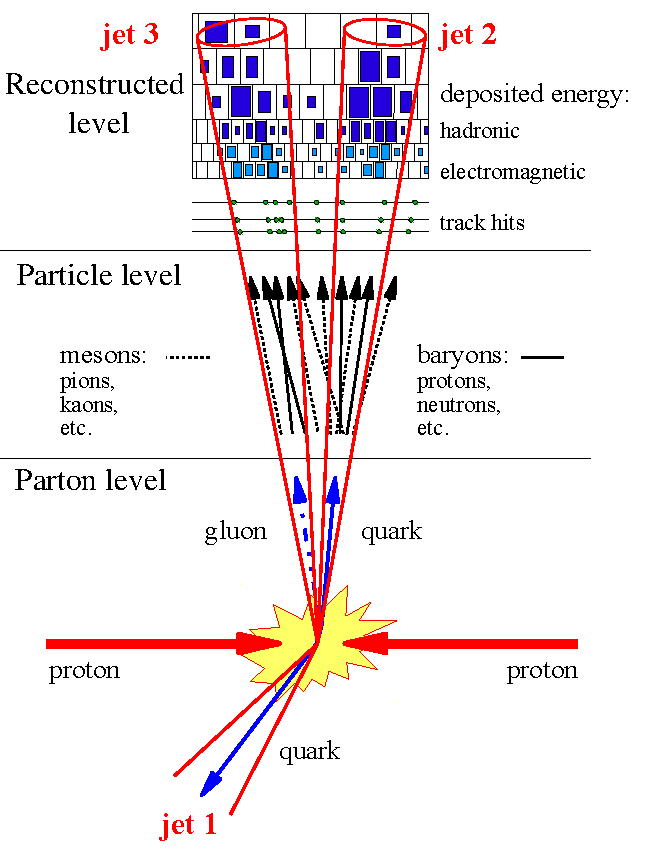
\includegraphics[scale = 0.95]{/home/anter/Desktop/Thesis/Figures/jet_levels_en_edited.pdf}\\
\vspace*{4mm}
\caption{In a proton-proton collision, the hard scattered quarks and gluons fragment and hadronize to produce the showers of partons, hadrons, or detector measurements which are clustered into parton jets, particle jets and reconstructed jets, respectively. Taken from \cite{Schorner-Sadenius:2015cga}.}
\label{fig:jets}
\end{center}
\end{figure}
{\bf Generator Jets -} The stable particles generated by the Monte Carlo event generators are clustered into generator jets (GenJets). At this particle level, the passage through the detector simulation has not been carried out. The objects at this level are charged hadrons, photons and neutral hadrons. Since the energy of GenJets is independent of the detector response, these are considered as reference objects for jet energy corrections. \\ \newline
{\bf Calorimetric Jets -} The jets reconstructed using the energy clusters deposited in the ECAL and HCAL calorimeter towers are called Calorimetric jets (CaloJets). One calorimetric tower consists of one HCAL cell surrounded by an array of 5 $\times$ 5 ECAL cells. The tower’s four- momenta are computed taking the direction from the interaction point to the tower center and assuming zero mass. All towers with a transverse-energy measurement above 300 MeV are considered in the clustering process. CaloJets are relatively simple objects because only calorimeter information is deployed, but they are strongly affected by the non-linearity of the calorimeter response. Since the readout of calorimeter measurements is fast, CaloJets are commonly used by the trigger system. \\ \newline
{\bf Particle Flow Jets -} The clustering of particle flow candidates give detector level jets called Particle Flow jets (PFJets). The four-momenta of the particles is taken as the input. The use of the tracking detectors and high granularity of the ECAL improves the energy resolution through the independent measurements of charged hadrons and photons inside a jet. Hence PFJets perform better than CaloJets and are the standard jets used at CMS.

The study presented in this thesis uses the jets clustered using the anti-\kt algorithm with a jet size parameter of R = 0.7 and particle flow candidates. In CMS, all the particles are reconstructed and identified using a Particle Flow (PF) algorithm, discussed in details in next section.  
%Each PFJet is matched to its corresponding GenJet topologically, by choosing the closest GenJet in $\eta$-$\phi$ plane. 

\subsection{Particle Flow Algorithm}
To identify and reconstruct the particles, the CMS employs the event reconstruction technique called Particle Flow (PF) algorithm \cite{CMS:2009nxa, CMS:2010byl}. Basically, the detector signals are concerted back to physical objects by using PF event reconstruction algorithm, as shown in Fig.~\ref{fig:PF_algo}. 
%http://inspirehep.net/record/1324461.}
It combines the information from the individual sub-detectors. The additional identification of the tracks, using the Combinatorial Track Finder (CTF) algorithm \cite{Adam:2005cg}, enhances the reconstruction performance. Based on these tracks, the primary vertices in an event are identified. The transverse momenta of final state stable particles or energies of the calorimeter towers are the inputs to PF algorithm. The PF algorithm first collects reconstructed hits in each sub-detector independently and creates a list of reconstructed elements (referred as blocks) : charged tracks in tracker, energy clusters in calorimeters and muon tracks in muon system. Then a link algorithm connects topologically compatible blocks producing PF objects. The PF objects consists of all stable particles : electrons, muons, photons, charged and neutral hadrons. The combination of the track momentum at the main interaction vertex, the corresponding ECAL energy deposit and the energy sum of all bremsstrahlung photons associated with the track is used to determine the energy of electrons. The curvature of the tracks in tracker and muon chamber is used to estimate the energy of muons.  The energy of photons is obtained directly from the ECAL measurement, corrected for zero-suppression effects\footnote{To suppress noise in the calorimeters, only cells with energies above a given threshold are considered and this procedure is known as zero-suppression.}. The energy of charged hadrons is calculated by combining the track momentum and corresponding energy clusters in ECAL and HCAL, corrected for zero-suppression effects as well as calibrated for the nonlinear response of the calorimeters. The energy of neutral hadrons is obtained from the corresponding calibrated ECAL and HCAL energies only. Along with the reconstruction of these objects, missing transverse energy (\ETmiss) is also determined using PF algorithm. \ETmiss is defined as the negative vector sum of transverse momenta \pt of all the isolated stable particles reconstructed in an event i.e. \ETmiss = $-\sum\limits_{\rm i}^{}\overrightarrow{p_{\rm T,i}}$. To avoid any kind of double-counting of energy, blocks of all PF reconstructed particle objects are removed and the energy of the calorimeter clusters is recalculated. Finally, the collection of PF objects is used to reconstruct the jets by using jet clustering algorithms. 

\begin{figure}[!t]
 \begin{center}
 \vspace*{4mm} 
 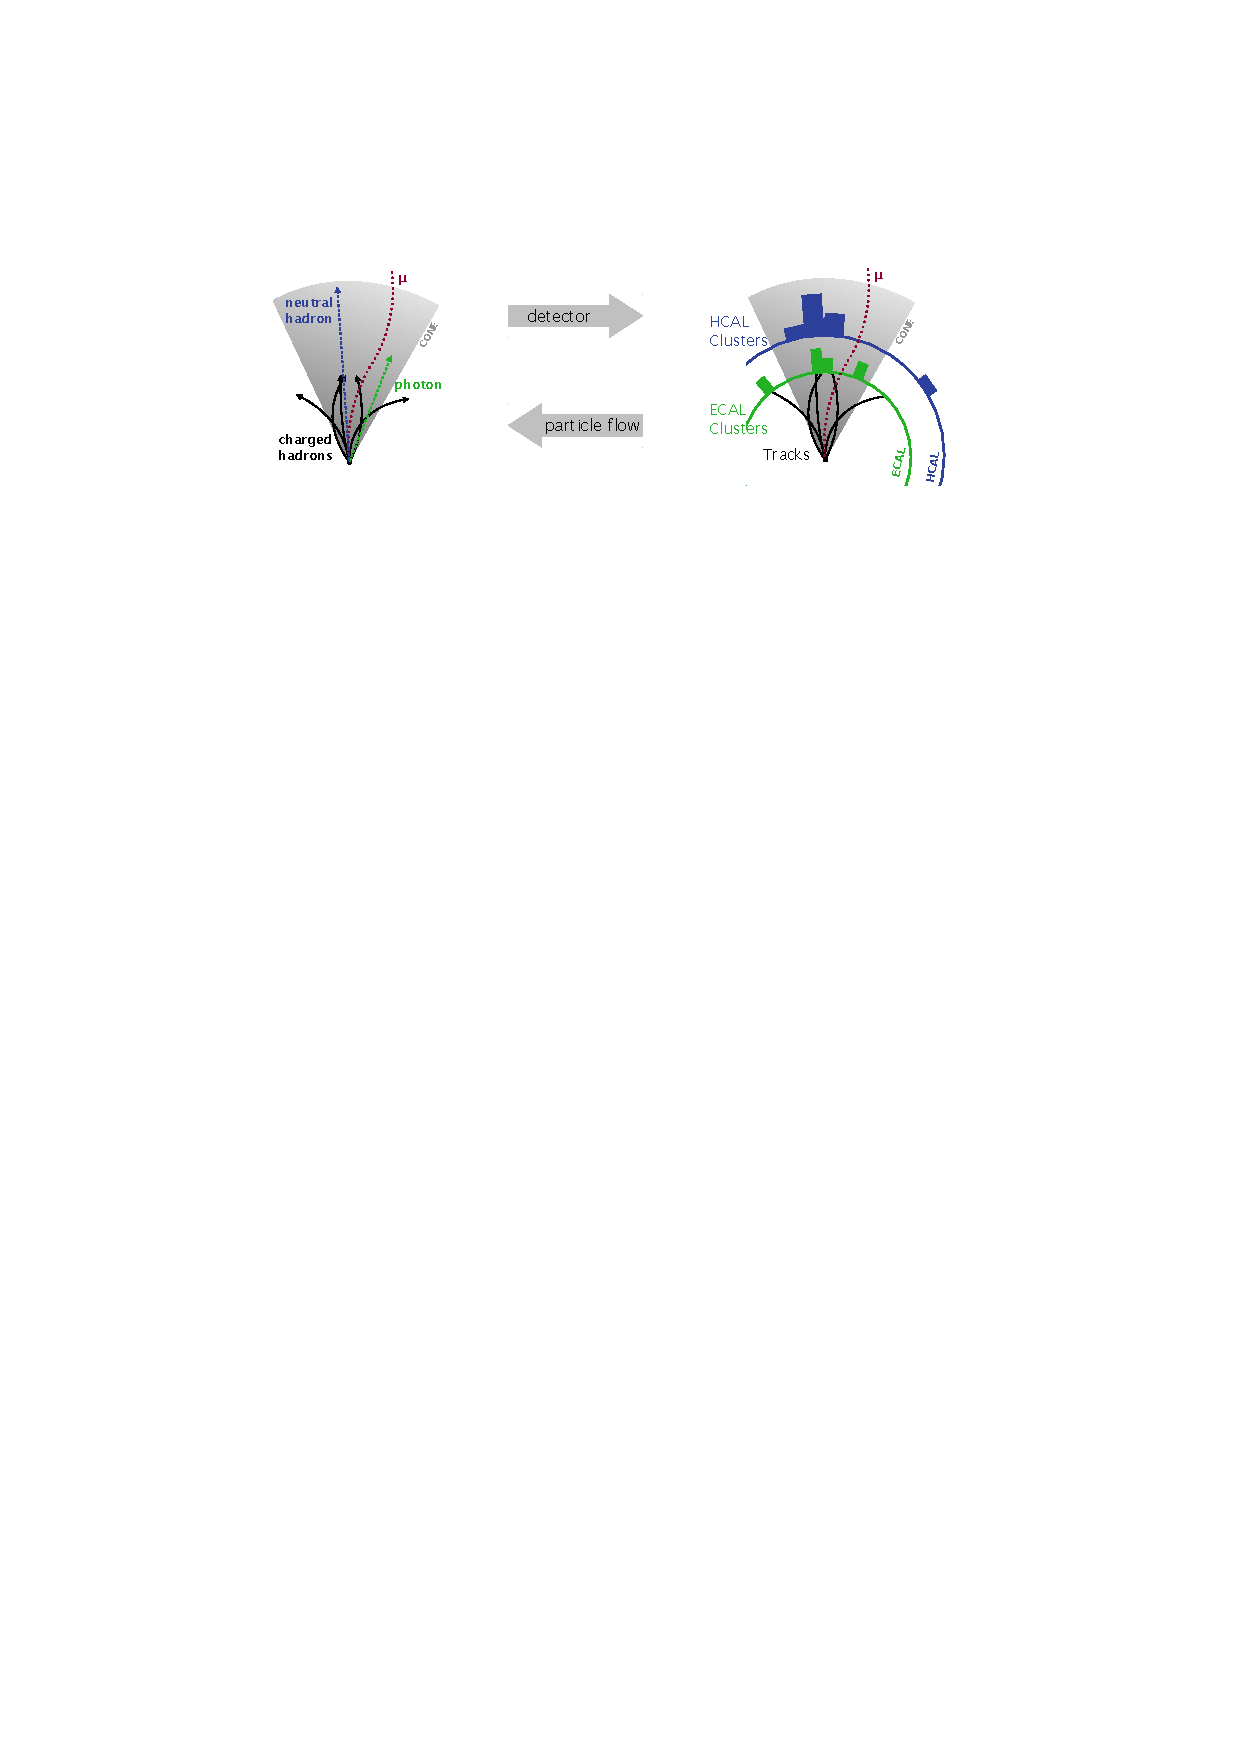
\includegraphics[width=1.\textwidth]{/home/anter/Desktop/Thesis/Figures/cropped_PF.pdf}
 \vspace*{5mm}
 \caption{Schematic association of sub-detector measurements to physical particle objects using the Particle Flow (PF) event reconstruction technique used by CMS. \cite{Rabbertz:2017ssq}}
 \label{fig:PF_algo}
 \end{center}
\end{figure}

\subsection{Jet Energy Corrections}
\label{sec:jet_corrections}
The measured energy of jets cannot be directly translated to the true particle or parton level. This is because of the nonlinear and nonuniform response of the calorimeters, effects of pileup and small residual effects in the data after corrections based on MC simulation. Hence to relate the measured jet energy to the corresponding true particle jet energy, jet energy corrections (JEC) \cite{Chatrchyan:2011ds, Khachatryan:2016kdb} are used to correct the measured jet energy. CMS follows a factorized approach, as presented in Fig.~\ref{fig:jec}, where JEC are applied in a sequential manner with fixed order, i.e. the output of one step serves as the input for the next one. Each level of correction takes care of a different effect and is independent of each other. At each step, the jet four momentum is scaled with a correction factor which depends on jet \pt, $\eta$, flavor etc.

\begin{figure}[!h]
 \begin{center}
 \vspace*{4mm} 
 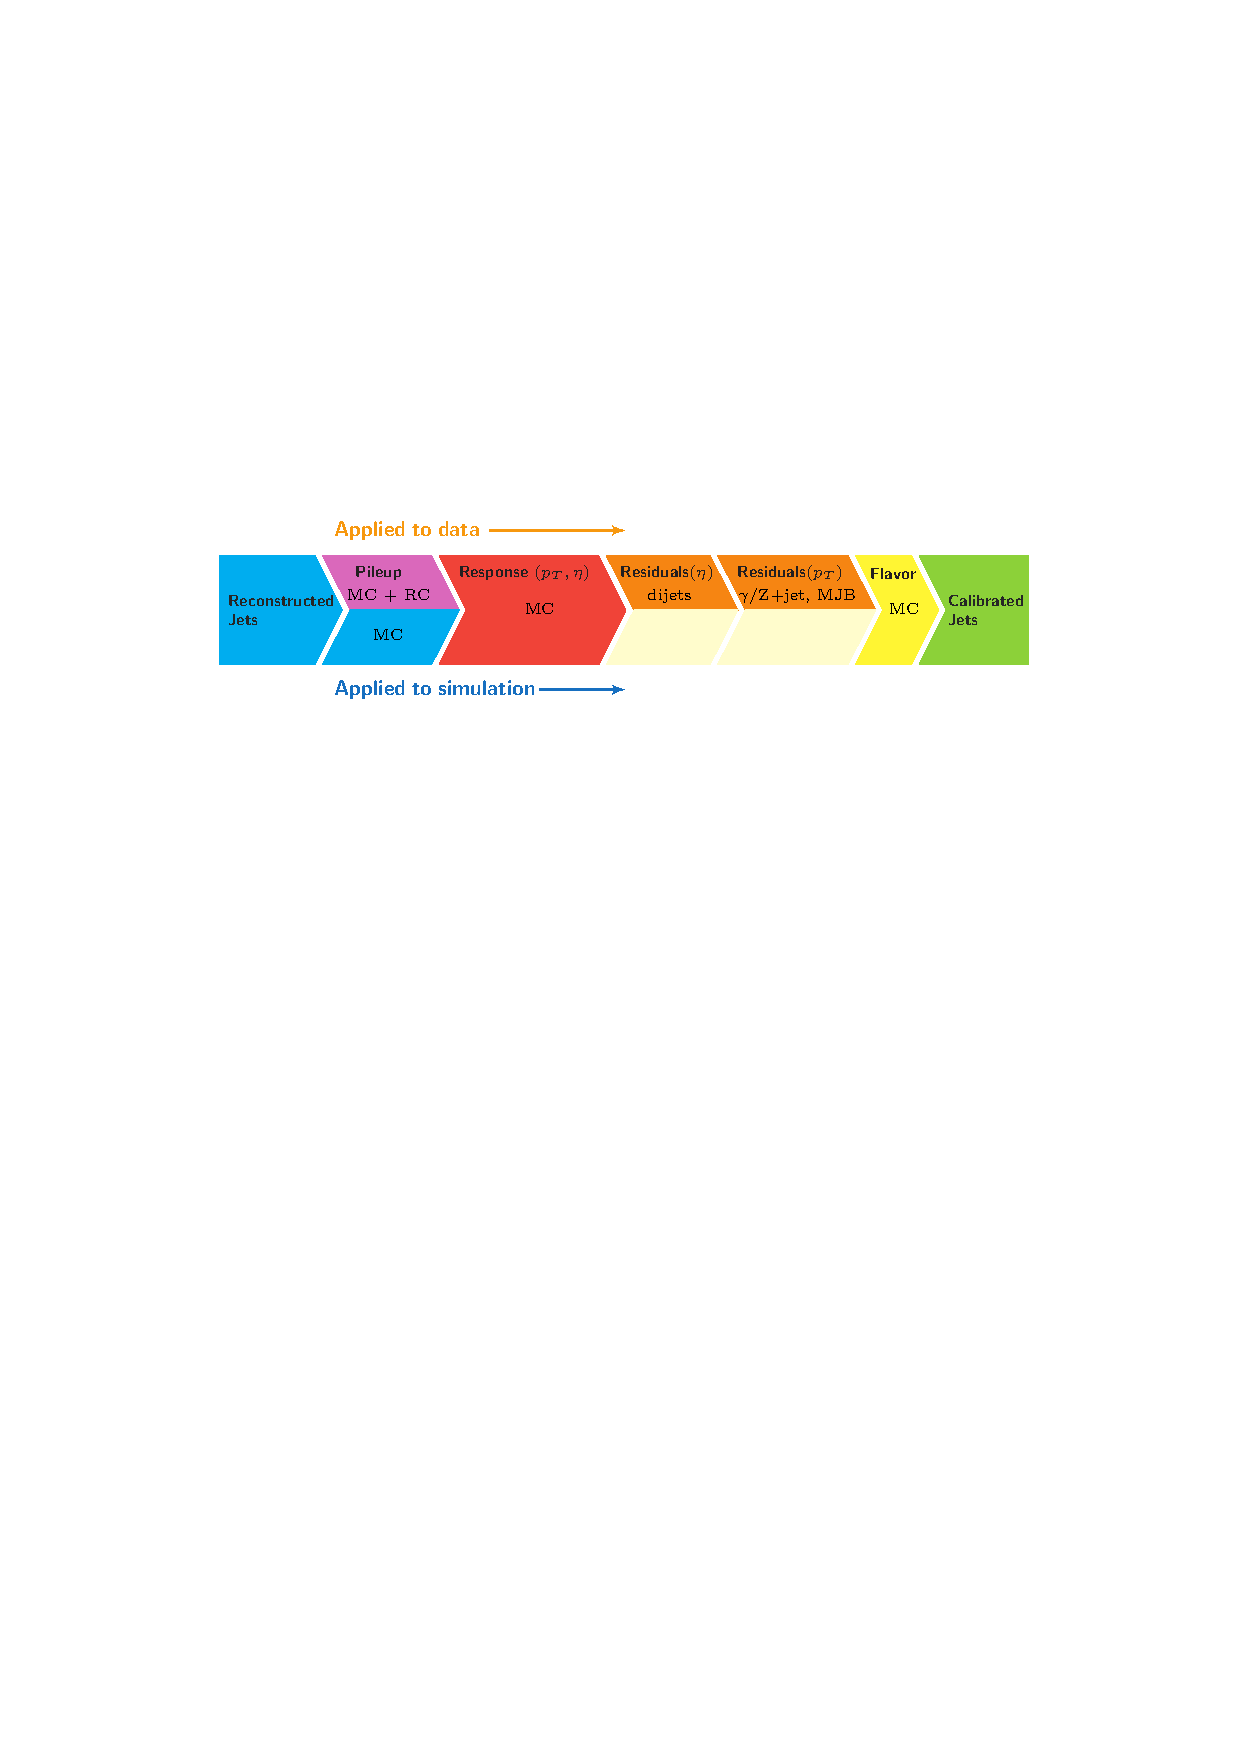
\includegraphics[width=1.\textwidth]{/home/anter/Desktop/Thesis/Figures/cropped_JEC.pdf}\\
 \vspace*{5mm}
 \caption[Lumi]{A schematic diagram of the factorized jet energy corrections (JEC) for data (upper half) and simulation (lower half) \cite{Khachatryan:2016kdb}. The reconstructed jets are corrected for pileup effects, non-uniform \pt and $\eta$ response and residual differences between data and Monte Carlo simulations along with optional flavor corrections. All corrections marked with MC are derived from simulation studies, RC stands for random cone, and MJB refers to the analysis of multijet events.}
 \label{fig:jec}
 \end{center}
\end{figure}

The corrected jet transverse momentum $p^{\rm corr}_{\rm T}$ is obtained by applying all correction factors subsequently on raw or uncorrected jet transverse momentum $p^{\rm raw}_{\rm T}$ as below :

\begin{equation}
p^{\rm corr}_{\rm T} = c_{\rm res}(\eta,p''_{\rm T})\cdot c_{\rm mc}(\eta,p'_{\rm T})\cdot c_{\rm pileup}(\eta,\rho,{\rm A}_{j},p^{\rm raw}_{\rm T})\cdot p^{\rm raw}_{\rm T}
\end{equation}
where $p'_{\rm T}$ is the transverse momentum after applying the pileup correction factor $c_{\rm pileup}$ on $p^{\rm raw}_{\rm T}$, $p''_{\rm T}$ is the transverse momentum after applying the additional correction factor $c_{\rm mc}$ because of relative and absolute effects derived from MC. At last a correction factor $c_{\rm res}$ for residual effects derived from data is applied. The corrections applied at each step are discussed as : \\\newline
{\bf Pileup Corrections -} The additional proton-proton collisions occurring within the same bunch-crossing produce particles which got clustered into the jets coming from the hard interaction. This extra energy must be subtracted from the reconstructed jet energy. This is done by applying the pileup corrections to raw jet $p^{\rm raw}_{\rm T}$. The pileup corrections are determined from the simulation of a sample of QCD dijet events processed with and without pileup effects. The pileup correction factor, $c_{\rm pileup}$ is calculated using jet area method from the pileup density $\rho$ in the event and the jet area ${\rm A}_{j}$and is parametrized as a function of $\rho$, ${\rm A}_{j}$, jet \pt and $\eta$. The corrections for residual differences between data and detector simulation as a function of eta are determined using the random cone (RC) method in zero-bias events. Hence the different pileup corrections are applied to data and MC. \\ \newline
{\bf MC Corrections -} The next correction applied to the pile up corrected jets is based on simulated QCD events. There are some differences between the reconstructed and generated jet \pt because of inefficiencies introduced by the detector simulation. The correction factor, $c_{\rm mc}$ is derived by comparing the measured jet \pt to the particle level jet \pt. The corrections are determined as a function of jet \pt and $\eta$ which make the detector response uniform over these two variables. \\ \newline
{\bf Residual Data Corrections -} The jets corrected with above mentioned corrections are further corrected for remaining small differences between data and Monte Carlo simulations. This correction is only applied to data. The correction factor $c_{\rm res}$ is derived using data-driven methods. The relative residual corrections are based on well-balanced dijet events in which a forward probe jet is calibrated using a tag jet in the well understood barrel region. The last correction step is the absolute residual correction in which reconstructed Z bosons balanced to a jet are used to calibrate the jet energy using the very precisely reconstructed Z boson. \\ \newline
{\bf Flavor Corrections -} These corrections correct the jets for flavor dependence (b, $\tau$ etc.) and are optional. These are extracted using Z\plusn jet and photon\plusn jets simulated events. The flavor corrections have not been applied for 8 TeV data.

The process of correction of jets by using JEC introduces uncertainties in the final corrected jet energy which are discussed in Sec.~\ref{sec:jecs_unc}.

\section{Software Tools}
Every year, the CMS is recording a huge amount of data, from collisions as well as simulations. This data is analyzed iteratively to improve the understanding of the detector and the measured physics. So a dedicated data structure and software tools are required for data analysis. These are included in the software framework referred to as CMSSW. This section describes the CMSSW framework and software tools used in the current study.

%CMSSW has also some pre-defined data tier, i.e sets with specific objects. Among them are the data tier RECO which included all reconstructed data objects, whereas the data tier AOD (Analysis Object Data) is only a subset with physical objects needed for a particular analysis.
\subsection{CMSSW Framework}
The CMS software framework (CMSSW) \cite{CMS:2005aa} provides all necessary tools for a physics analysis. The CMSSW framework is built on top of an event data model (EDM). It is a container for arbitrary C\plusn\plus objects, e.g. recorded raw data and reconstructed physical objects (e.g particles, missing transverse energy) or derived quantities of an event. The reconstruction and distribution algorithms in CMSSW are divided into modules, which can be dynamically loaded and run. The CMSSW event processing model consists of one executable, called cmsRun, and many plug-in modules which are managed by the framework. SCRAM (Source Configuration, Release, And Management) is a configuration and management tool in the framework. It builds a runtime environment and make available all the necessary shared libraries. The shared libraries reduces memory consumption by only loading required modules during runtime. The CMSSW framework performs calibration, event generation, detector simulation, event reconstruction as well as data analysis by implementing the codes either in C\plusn\plus or Python languages. To reduce the event content, a process called skimming is performed where only necessary data is preserved. 

\subsection{ROOT}
ROOT \cite{Brun:1997pa} is an object-oriented data analysis framework, developed by CERN. ROOT consists of a huge C\plusn\plus library provided with all the functionalities to store and analyze large amounts of data. It provides histrogramming methods in 1, 2 and 3 dimensions, curve fitting, function evaluation, minimization, graphics and visualization classes. The command language of ROOT is command line interpreter (CINT), with several extensions to C\plusn\plus which makes ROOT a versatile package. ROOT is an open-source system which can be dynamically extended by linking external libraries. The events generated or analyzed in CMSSW framework are stored in a tree structure in files using ROOT libraries. In this thesis, ROOT has been used extensively for storing information of events or objects, for fitting as well as plotting purposes.
